\documentclass{article}
\usepackage[utf8]{inputenc}
%\usepackage{natbib}
\usepackage{graphicx}
\usepackage{hyperref}
\usepackage{color}
\usepackage{listings}
%\usepackage{lastpage}
\usepackage{wrapfig}
%\usepackage{eso-pic}
%\usepackage{tikz}
\usepackage{float}
\usepackage{amssymb}
\usepackage{caption}
\usepackage{subcaption}
%\usepackage{pdfpages}
\usepackage[backend=biber]{biblatex}
\definecolor{commentgreen}{RGB}{100, 190, 100}
\definecolor{gray}{RGB}{50, 50, 50}
\lstset{language=C,
                breaklines=true,
                basicstyle=\ttfamily\scriptsize,
                keywordstyle=\color{blue}\ttfamily,
                stringstyle=\color{red}\ttfamily,
                commentstyle=\color{commentgreen}\ttfamily,
                morecomment=[l][\color{magenta}]{\#},
                numberstyle=\tiny\color{gray},
                numbers=left
}


\title{IP - Mini-project:\\Topic 6: Convert from RGB to HSI}
\author{Jannick Drews}
\date{\today}

\newcommand{\secref}[1]{\nameref{#1}~\ref{#1}}
\newcommand{\goodcite}[1]{\textsuperscript{\cite{#1}}}

\addbibresource{Ref.bib}

\setlength\parindent{0pt}
% Each student makes a document that contains -----
% 1) an explanation of their algorithm,
% 2) their code,
% 3) an explanation of their code and 4) a documentation of the program (show input and output) and showing the effect of different parameters on the algorithm, if any.
% Everything is collected in ONE PDF file per student. The document should be named like this: ”your topic_your name#”.pdf
% group presentation can be just the PDF

%Each project must as a minimum contain
% variables
% a function (main() does not count),
% a loop, and an
% if-else statement
%example to rotate an image, but it is fine to use Op

% forward and backward mapping(find out yourself)

%randomizationphase


%  My: Topic #6: Convert from RGB to HSI
% Everything in one PDF file (describe topic(explain what it is, how its performed), then add my own code and description of the code(line by line or part by part))(Whats input and whats output)

\begin{document}
\pagenumbering{gobble}
\maketitle
\newpage
\pagenumbering{arabic}

\section{Convert from RGB to HSI}
The \texttt{RGB} and \texttt{HSI} refers to their respective color-spaces. These are used to display an image in a certain aspect, both color-spaces presented in a digital form will use a 3-dimensional array.\\
For \texttt{RGB}, the 3-dimensional array would look like the following; $[R, G, B]$, an example could be $[255, 10, 25]$ which is the value 255 for the red channel, 10 for the green channel and 25 for the blue channel. Note that RGB values follow the ruleset\goodcite{IP}; $$ R,G,B \in [0, 255] $$\\
For the \texttt{HSI} color-space, represented digitaly it would look like; $[H, S, I]$, an example could be $[310, 0.3, 144]$ which is the value 310 for the hue in degrees, 0.3 for the saturation and 144 for the intensity. Note that HSI values follow the ruleset\goodcite{IP}: $$ H \in [0, 360[ $$ $$ S \in [0, 1]$$ $$ I \in [0, 255]$$ Keep in mind that this color-space does have a inconsistent naming convention, it is also known as \texttt{HSB} and \texttt{HSL}, if not more.\medskip \\
This assignment will convert the RGB color-space to the HSI color-space, this is performed by utilizing the formulas found on \autoref{fig:formulas} \goodcite{IP}
\begin{figure}[H]
    \centering
    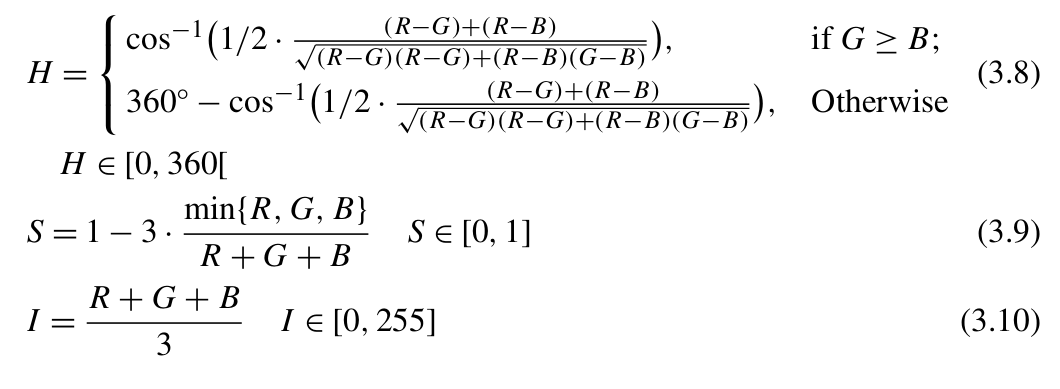
\includegraphics[width=\textwidth]{img/formula.png}
    \caption{Formulas for converting RGB to HSI\goodcite{IP}}
    \label{fig:formulas}
\end{figure}
For converting the degrees to radians and vice versa;
\begin{figure}[H]
    \centering
    $$ D_{deg} = R_{rad} \cdot \frac{180}{\pi},\ R_{rad} = (\frac{D_{deg}}{180}) \cdot \pi $$
    \caption{Radians $\rightarrow$ Degrees and Degrees $\rightarrow$ Radians}
    \label{fig:convert}
\end{figure}
And the description of the assignment is the following:\\
\textit{"Make a Python program that can convert from RGB to HSI.\\Input: An RGB image\\Output: Three images: a H-image, a S-image, and an I-image"}
% How its performed ??

\section{Implementation}
\subsection{Code \& Description}
Following is my implementation of the channel conversion from RGB to HSI:
\lstinputlisting[language=Python]{miniproject.py}

\underline{Lines; 7 to 10} % Copy + 3 channels
A copy of the image is made, to show later for comparison. 3 different channels(matrices) are made for h,s,v respectively, hence the naming convention. These 3 new channels are of the same shape of the original image, and has a depth value of a float32 since float numbers are going to be present in the Saturation channel.\medskip \\
\underline{Lines; 11 to 17} % For loop & grab values
Inside a double for-loop, to go through each pixel in the image, we grab the respective colors from the red, green and blue channel of the input image, and store them as integers to be sure the calculations will be done properly.\medskip \\
% MENTION IT FUCKED?
\underline{Lines; 20 to 39} % Calculate formula for H, only partly + exception
The different variables are assigned to the respective parts of the formula from \autoref{fig:formulas}, and makes sure to catch the exception where $R = G = B$. And lastly the \texttt{formula} variable calculates the remaining part of the formula. The \texttt{top} variable calculates the top part of the formula, and the \texttt{bot} calculates the bottom part.\\
We then check if the statement from the formula is true, that if $ G \ge B$ then we subtract 360 degrees, and remember to convert it first to $2\cdot\pi$ for the radians.\\
And the last instruction converts the radian back to degrees.\medskip \\
%%%%%%%%%%%%%%%%%%%%
% REFERENCE THE CONVERSION ??%
%%%%%%%%%%%%%%%%%%%%
\underline{Lines; 43 to 54}
From here we calculate the Saturation and the Intensity channels, still following the formula described at \autoref{fig:formulas}.
First the saturation, which is dividing the minimum value of the respective red green or blue channel, this formula is also split it for ease of reading.\\
Lastly the intensity channel is calculated by finding the mean of the R,G,B pixels. And lastly put into the respective HSI channels.
\underline{Lines; 57 to 66}
These lines just serve to subplot the images and display the different resulting HSI channels in comparison to the original RGB image.\medskip \\
\underline{Lines; 69 to 74}
This function just convers the BGR to RGB image, since OpenCV loads as BGR first, I had to do a convert to RGB previously to inputting the image into the main function to convert to HSI. This function just creates a new temporary channel to store the red, and then it switches the blue and red channel with eachother to get RGB.\\
\underline{Lines; 76 to 78}
These three lines just load the image and convert it to RGB and put it into the HSV conversion function.\\
% Description of code (line by line, part by part)

% Whats input and whats output
\subsection{Input/Output}
The subplot illustrated on \autoref{fig:subplot}, is displayed after the code has executed, where the \textit{"Original"} is the original RGB image, of cause converted to RGB with the conversion function implemented at line \texttt{69}, and the rest of the titles are the Hue, Saturation and Intensity channels respectively.
\begin{figure}[H]
    \centering
    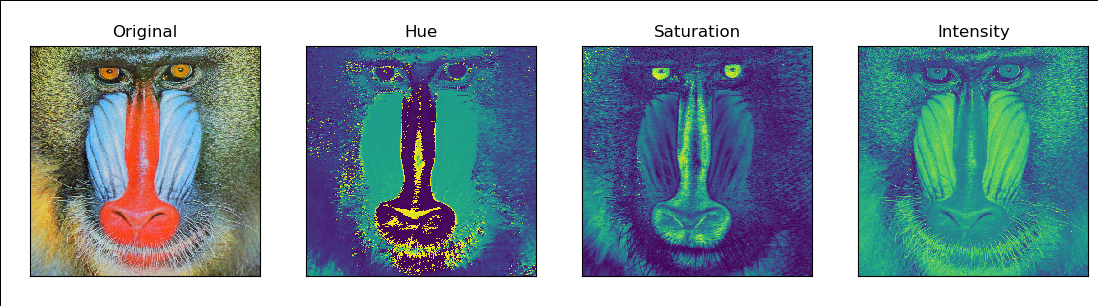
\includegraphics[width=\textwidth]{img/output.png}
    \caption{Subplot result from code}
    \label{fig:subplot}
\end{figure}
\section{Points of note}
% PROOF OF CALCULATIONS CROSS-REFERENCE
As illustrated on \autoref{fig:subplot}, the \textit{"Hue"} channel may look weird, theoretically this could be a display error from matplotlib, since it potentially does not know how to handle the values from; $]255, 360 [$. The reason for writing this section is to portray that the resulting calculations from the implementation are indeed correct.\\
The next figures will illistrate calculations from Wolfra Alpha, which is a huge computational system that has features such as; solving math equations. I will compare the results from Wolfram Alpha with my implementations results.

\begin{figure}[H]
\centering
\begin{subfigure}{.5\textwidth}
  \centering
  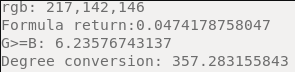
\includegraphics[width=0.9\linewidth]{img/rgb-217-142-146-code.png}
    \caption{Result from implementation}
  \label{fig:217_code}
\end{subfigure}%
\begin{subfigure}{.5\textwidth}
  \centering
  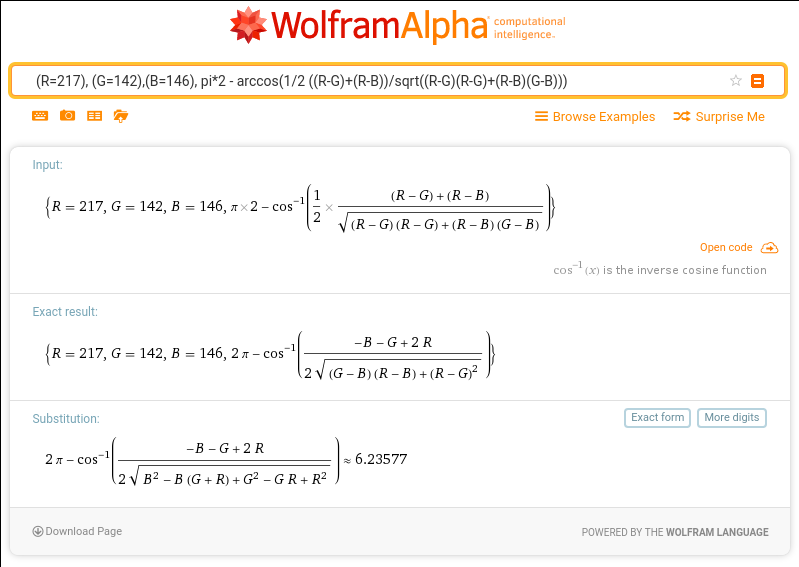
\includegraphics[width=0.9\linewidth]{img/rgb-217-142-146-wolfram.png}
    \caption{Result from Wolfram alpha\goodcite{Wolfram}}
  \label{fig:217_wolfram}
\end{subfigure}
\caption{Comparison of implementation result and wolfram alphas result}
\label{fig:Comparison-217}
\end{figure}

\begin{figure}[H]
\centering
\begin{subfigure}{.5\textwidth}
  \centering
  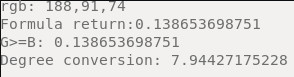
\includegraphics[width=0.9\linewidth]{img/rgb-188-91-74-code.png}
    \caption{Result from implementation}
  \label{fig:188_code}
\end{subfigure}%
    \begin{subfigure}{.5\textwidth}
  \centering
  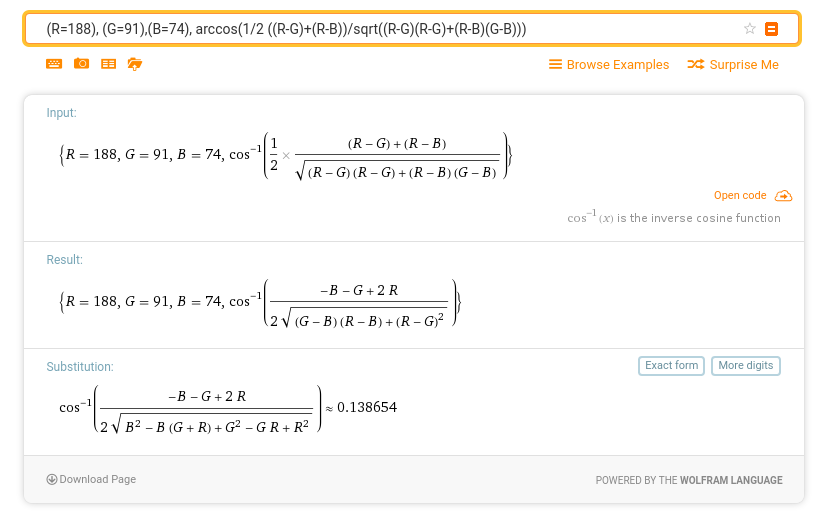
\includegraphics[width=0.9\linewidth]{img/rgb-188-91-74-wolfram.png}
    \caption{Result from Wolfram alpha\goodcite{Wolfram}}
  \label{fig:188_wolfram}
\end{subfigure}
    \caption{Comparison of implementation result and wolfram alphas\goodcite{Wolfram} result}
\label{fig:Comparison-188}
\end{figure}

\autoref{fig:Comparison-217} and \autoref{fig:Comparison-188}, shows the results from my implementations calculations and the calculations done by Wolfram alpha\goodcite{Wolfram} for the Hue value, using the Hue formula from \autoref{fig:formulas}, the difference of the two figures being the boolean $G \ge B$. Both get the same result for the Hue value, which stands to show that the calculations for the pixel values in the Hue channel are correct, but also stands to show that the display may be incorrect. As mentioned before, this could be a result of matplotlib displaying the channel incorrectly(Which seems improbable) or a bug.

\newpage
\section{Bibliography}
\printbibliography


\end{document}

